%% appendix.tex
%%

\chapter{Appendix}
\label{ch:Appendix}

\section{Autoencoder-Architekturen und Trainingsdetails}
\label{ch:Appendix:Architektur-Details}
In diesem Abschnitt werden Details zu den Autoencoder-Architekturen und Details zum Training der Autoencoder erläutert. Zuerst werden die Architekturen der klassischen vollvernetzten Autoencoder (AE), dann die Architekturen der Convolutional Autoencoder (ConvAE) und zuletzt die Architektur der Contractive Autoencoder (CAE) spezifiziert. Anschließend wird der benutzte Optimierer und andere Trainings-Details genannt. Da die Architekturen
vom Datensatz abhängen, werden diese in folgender Tabelle nach dem Datensatz gruppiert.

\ldots

Alle Autoencoder werden mit dem \textit{PyTorch}-Framework implementiert, wobei \textit{Skorch} für
die Kompatibilität mit anderen \textit{Scikit-Learn} Algorithmen eingesetzt wird. Als Optimierer
wird \textit{Adam} eingesetzt, der häufig für das Trainieren neuronaler Netze gegenüber anderen
Optimierern wie \textit{Stochastic Gradient Descent} (SGD) präferiert wird. Die Lernrate $\eta$
wird mittels eines exponentiellen Verfalls nach jeder Epoche aktualisiert. Dazu wird $\eta$ nach
jeder Epoche $t = 1, \ldots, t_{\text{max}}$ mit einem Wert $\gamma$ multipliziert. Dieser Wert
wird für alle Autoencoder auf $\gamma = 0,9$ gesetzt. Die klassischen und Contractive Autoencoder
werden für maximal 100 Epochen und die Convolutional Autoencoder für maximal 150 Epochen trainiert.
Das Training wird frühzeitig beendet, wenn sich der Validierungsfehler innerhalb von 20 Epochen
nicht mehr verbessert. Die Größes eines Batches ist datensatzabhängig nach Stichprobengröße gewählt
worden und beträgt 32 für Swiss Roll und Twin Peaks, acht für Olivetti Faces und ICMR, 100 für
MNIST und FER-2013 und 64 für LfwPeople.

\section{Qualitätskriterien für die Datensätze}
\label{ch:Appendix:Qualitaetskriterien}

In diesem Abschnitt werden die Abbildungen der Qualitätskriterien für die restlichen Datensätze
gesammelt. In \figref{fig:TwinPeaksMetrics} sind die Qualitätskriterien für die Twin Peaks, in
\figref{fig:ICMRMetrics} die Qualitätskriterien für ICMR, in \figref{fig:OlivettiFacesMetrics} die
Qualitätskriterien für den Olivetti Faces Datensatz, in \figref{fig:LfwPeopleMetrics} für den
LFW-atensatz und in \figref{fig:FER2013Metrics} für den FER-Datensatz.
\begin{figure}[ht]
	\begin{center}
		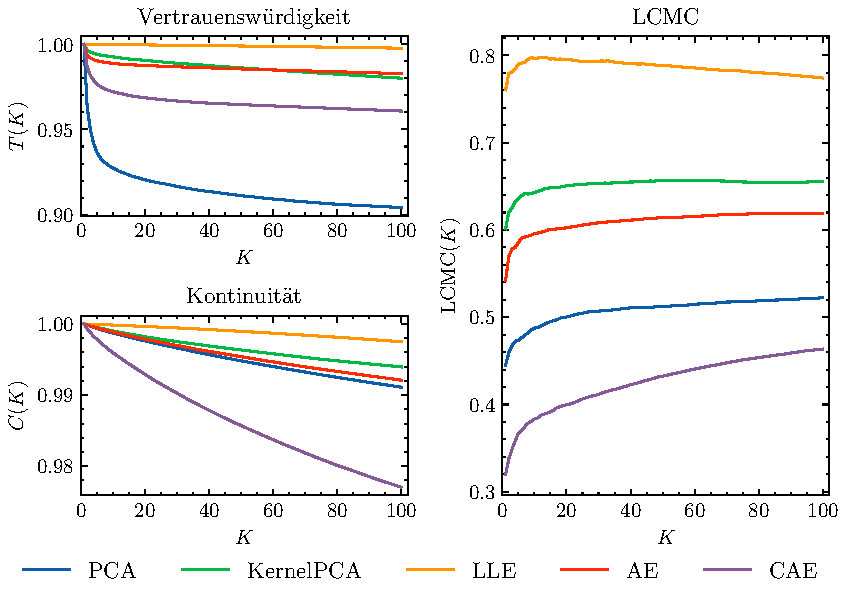
\includegraphics{TwinPeaks_comparison.pdf}
	\end{center}
	\caption[Qualitätskriterien für die Twin Peaks]{Die Vertrauenswürdigkeit und Kontinuität der Dimensionsreduktion, sowie das Local Continuity Meta-Criterion (LCMC) für den Twin Peaks Datensatz. Locally Linear Embedding (LLE) schneidet wie bei der Swiss Roll insgesamt am besten ab, dicht gefolgt vom Autoencoder und der Kernel PCA. Lediglich der Contractive Autoencoder (CAE) und PCA fallen auf diesem künstlichen Datensatz etwas zurück, wobei die Vertrauenswürdigkeit der Dimensionsreduktion von PCA deutlich schlechter als bei den restlichen Methoden ist. Dies ist höchstwahrscheinlich der nichtlinearen Mannigfaltigkeit geschuldet, was der linearen Hauptkomponentenanalyse Schwierigkeiten bereitet. (Eigene Darstellung)}
	\label{fig:TwinPeaksMetrics}
\end{figure}

\begin{figure}[ht]
	\begin{center}
		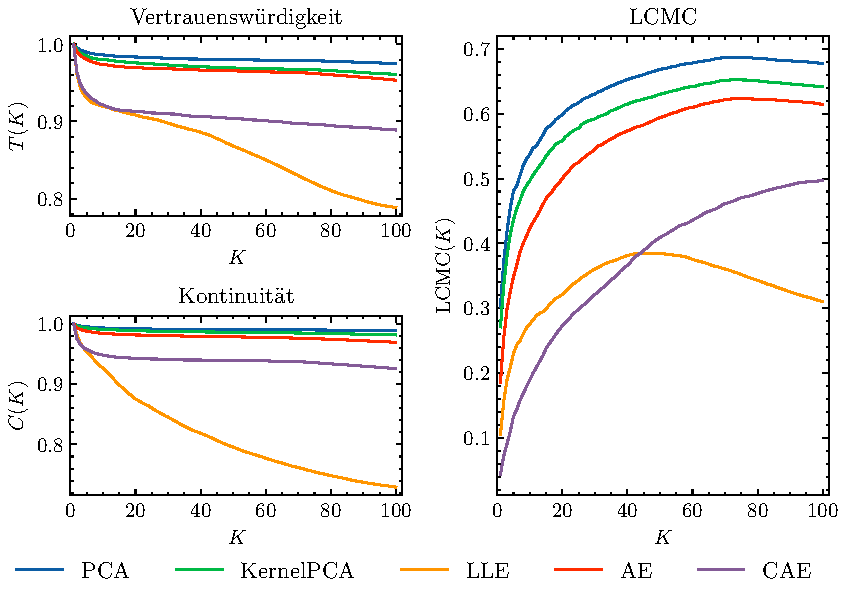
\includegraphics{ICMR_comparison.pdf}
	\end{center}
	\caption[Qualitätskriterien für den ICMR-Datensatz]{Die Vertrauenswürdigkeit und Kontinuität der Dimensionsreduktion, sowie das Local Continuity Meta-Criterion (LCMC) für den ICMR-Datensatz. Dieser Datensatz ist kein Bilddatensatz, weswegen hier der Convolutional Autoencoder nicht eingesetzt werden konnte. Auch hier schneidet die Hauptkomponentenanalyse wieder am besten ab, gefolgt vom vollvernetzten Autoencoder (AE) und der Kernel PCA. Am schlechtesten sind der Contractive Autoencoder und Locally Linear Embedding. (Eigene Darstellung)}
	\label{fig:ICMRMetrics}
\end{figure}

\begin{figure}[ht]
	\begin{center}
		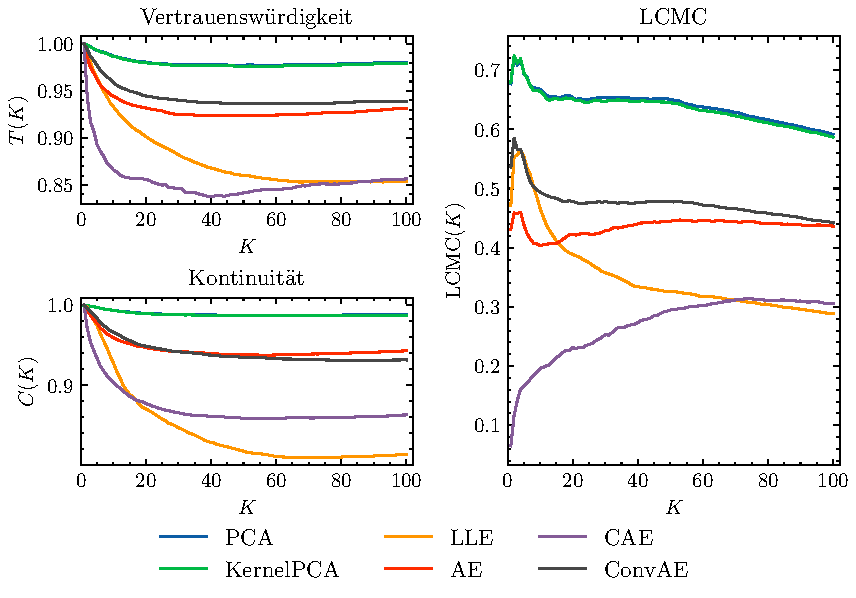
\includegraphics{OlivettiFaces_comparison.pdf}
	\end{center}
	\caption[Qualitätskriterien für den Olivetti Faces-Datensatz]{Die Vertrauenswürdigkeit und Kontinuität der Dimensionsreduktion, sowie das Local Continuity Meta-Criterion (LCMC) für den Olivetti Faces Datensatz. Hier schneiden alle Varianten der Autoencoder nicht so gut ab, wie es beispielweise auf dem MNIST Datensatz der Fall war. Dies könnte an der deutlich geringeren Stichprobengröße von 400 liegen, wodurch eine Konvergenz der Autoencoder schwieriger wird. Neben den Autoencoder schneidet hier auch LLE für größere Werte von $K$ schlecht ab, kann jedoch bei geringeren Nachbarschaftsgrößen hohe Werte für die Vertrauenswürdigkeit und Kontinuität erreichen. PCA schneidet hinsichtlich allen drei Kriterien für alle Werte von $K$ am besten ab, gefolgt von der Kernel PCA. (Eigene Darstellung)}
	\label{fig:OlivettiFacesMetrics}
\end{figure}

\begin{figure}[ht]
	\begin{center}
		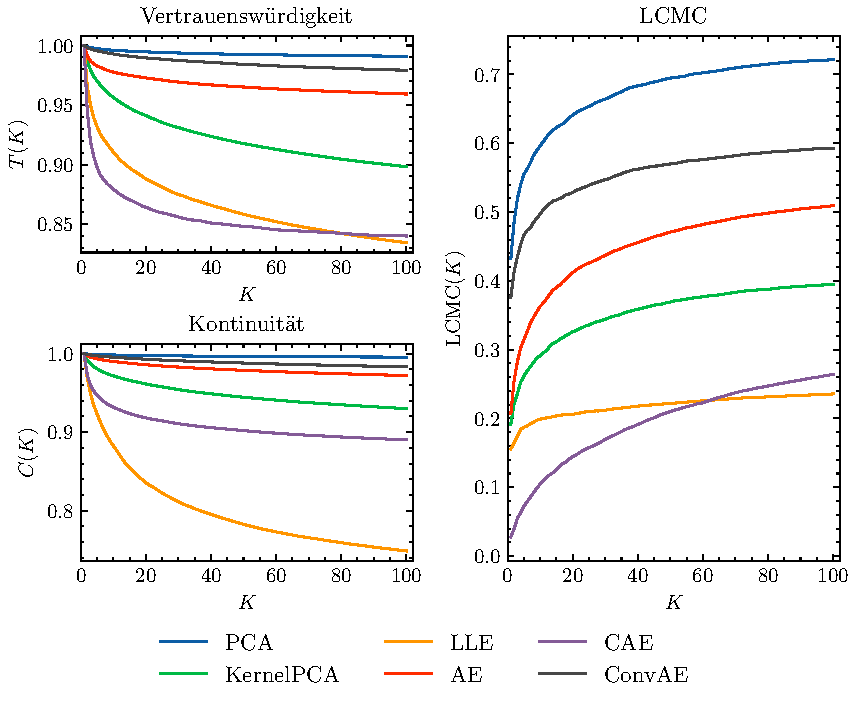
\includegraphics{LfwPeople_comparison.pdf}
	\end{center}
	\caption[Qualitätskriterien für den LFW-Datensatz]{Die Vertrauenswürdigkeit und Kontinuität der Dimensionsreduktion, sowie das Local Continuity Meta-Criterion (LCMC) für den LFW-Datensatz. Die Kriterien auf diesem Datensatz zeigen ein ähnliches Bild wie auf dem Olivetti Faces Datensatz, jedoch bereitet hier die Stichprobengröße keine Probleme beim Trainieren der Autoencoder. Daher können auch der Autoencoder und der Convolutional Autoencoder wieder eine bessere Performance aufweisen. Trotzdem ist auch hier die Hauptkomponentenanalyse wieder für alle Werte der Nachbarschaftsgröße am besten. (Eigene Darstellung)}
	\label{fig:LfwPeopleMetrics}
\end{figure}

\begin{figure}[ht]
	\begin{center}
		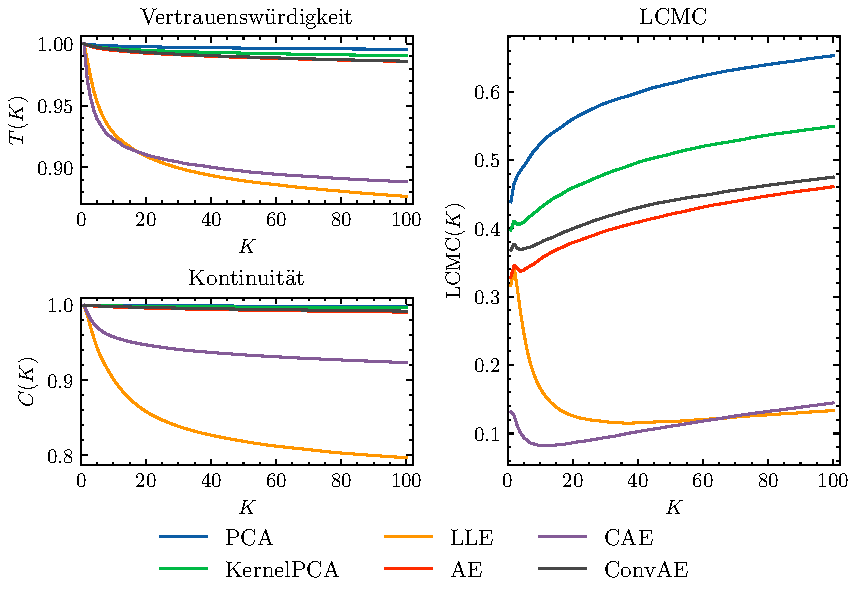
\includegraphics{FER2013_comparison.pdf}
	\end{center}
	\caption[Qualitätskriterien für den FER-Datensatz]{Die Vertrauenswürdigkeit und Kontinuität der Dimensionsreduktion, sowie das Local Continuity Meta-Criterion (LCMC) für den FER-Datensatz. Hier ist die Performance des Convolutional Autoencoders und der Hauptkomponentenanalyse nahezu identisch und im Vergleich mit den anderen Methoden am besten. Aber auch der Autoencoder und die Kernel PCA können einen konstant hohen Wert für $T(K)$ und $C(K)$ erreichen. Auch auf diesem Datensatz schneiden LLE und der Contractive Autoencoder mit Abstand am schlechtesten ab. Besonders LLE zeigt hier die Schwäche einer lokalen Erhaltung der Struktur, da die Qualitätskriterien für steigende Werte von $K$ stark abfallen. (Eigene Darstellung)}
	\label{fig:FER2013Metrics}
\end{figure}